\documentclass{article} % For LaTeX2e
\usepackage[submission]{colm2025_conference}

\usepackage{microtype}
\usepackage{hyperref}
\usepackage{url}
\usepackage{booktabs}

\usepackage{lineno}
\usepackage{graphicx}
\usepackage{tcolorbox}
\usepackage{tikz}
\usetikzlibrary{positioning, fit, arrows.meta, shapes.geometric}
\usepackage{wrapfig}
\usepackage{colortbl} % For row coloring

\definecolor{darkblue}{rgb}{0, 0, 0.5}
\hypersetup{colorlinks=true, citecolor=darkblue, linkcolor=darkblue, urlcolor=darkblue}


\title{AutoLibra \protect
\includegraphics[height=1em]{figs/scale.png} \\ \textit{Metric Induction for Agents from Open-Ended Human Feedback}}

% Authors must not appear in the submitted version. They should be hidden
% as long as the \colmfinalcopy macro remains commented out below.
% Non-anonymous submissions will be rejected without review.

\author{Antiquus S.~Hippocampus, Natalia Cerebro \& Amelie P. Amygdale \thanks{ Use footnote for providing further information
about author (webpage, alternative address)---\emph{not} for acknowledging
funding agencies.  Funding acknowledgements go at the end of the paper.} \\
Department of Computer Science\\
Cranberry-Lemon University\\
Pittsburgh, PA 15213, USA \\
\texttt{\{hippo,brain,jen\}@cs.cranberry-lemon.edu} \\
\And
Ji Q. Ren \& Yevgeny LeNet \\
Department of Computational Neuroscience \\
University of the Witwatersrand \\
Joburg, South Africa \\
\texttt{\{robot,net\}@wits.ac.za} \\
\AND
Coauthor \\
Affiliation \\
Address \\
\texttt{email}
}

% The \author macro works with any number of authors. There are two commands
% used to separate the names and addresses of multiple authors: \And and \AND.
%
% Using \And between authors leaves it to \LaTeX{} to determine where to break
% the lines. Using \AND forces a linebreak at that point. So, if \LaTeX{}
% puts 3 of 4 authors names on the first line, and the last on the second
% line, try using \AND instead of \And before the third author name.

\newcommand{\fix}{\marginpar{FIX}}
\newcommand{\new}{\marginpar{NEW}}

\begin{document}

\ifcolmsubmission
\linenumbers
\fi

\maketitle

\begin{abstract}
The evaluation and optimization of language agents are often based on either
task success or heuristically designed metrics.
However, these approaches are either not fine-grained enough or require 
manual design of the metrics by experts.
We propose \emph{AutoLibra},
a system that transforms human feedback, 
\emph{e.g.} ``\textsf{If you find that the button is disabled, don't click it again}'',
or ``\textsf{This agent has too much autonomy to decide what to do on its own}''
into metrics evaluating similar failure and successful modes.
AutoLibra accomplishes this by first grounding the feedback in the agent's behavior,
clustering similar positive and negative behaviors,
and creating metrics that are ready to prompt LLM-as-a-Judge with
concrete examples and definitions. 
We propose two \emph{meta metrics} to evaluate how aligned a set of (induced) metrics
is with human open-ended feedback: ``coverage'' and ``redundancy''.
Through optimizing these meta metrics, we find that AutoLibra could
not only recover the \textbf{agent evaluation} dimensions heuristically proposed
in previous agent evaluation benchmarks, but also discover the ones that have been overlooked.
Beyond agent evaluation, we demonstrate two practical applications of
AutoLibra in \textbf{agent improvement}:
First, we show that AutoLibra effectively selects high-quality agent fine-tuning data
for web browsing. Second, we demonstrate that the metrics extracted by AutoLibra serve
as better optimization targets than task success rate on two challenging text game tasks,
enhancing prompt engineering.
Our results suggest that AutoLibra can use very small number of annotations (less than 100 annotations), 
to induce a set of interpretable metrics with higher than 80\% coverage on unseen feedback.
\end{abstract}


\section{Introduction}

\begin{wrapfigure}[18]{r}{0.45\textwidth}
   \vspace{-40pt}
   \centering
   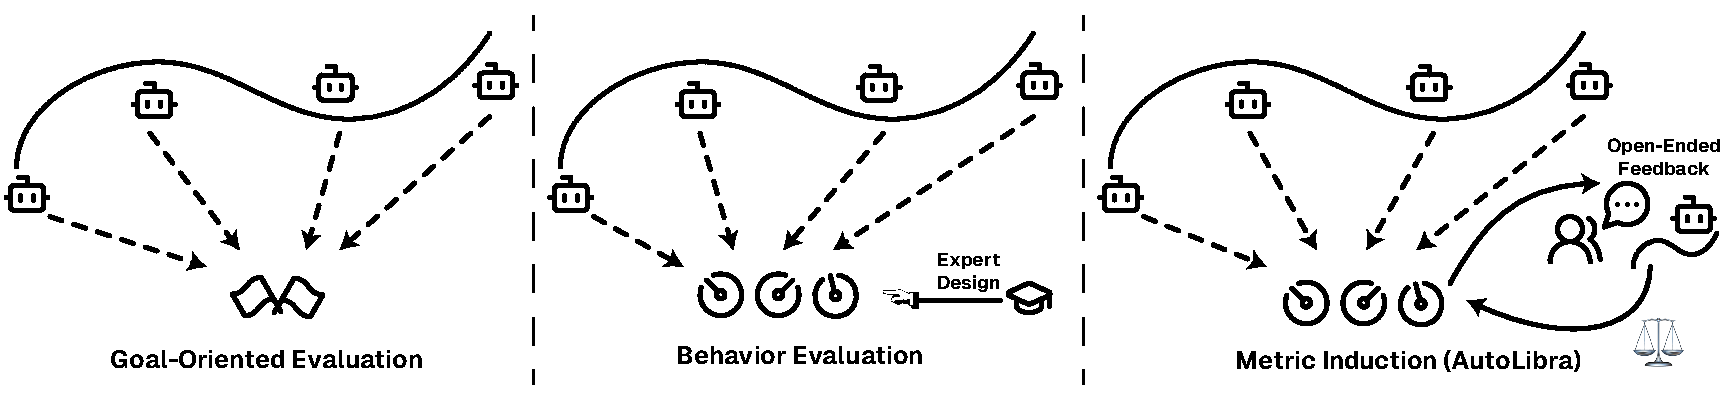
\includegraphics[width=0.45\textwidth]{figs/autolibra.pdf}
   \caption{AutoLibra provides behavioral evaluation on agent performance
    through automatic metric induction based on human feedback and agent trajectories.}
\end{wrapfigure}


Efficient human learners internalize open-ended feedback from others into self-regulation metrics
\citep{pintrich2002development,nicol2006formative}.
These metrics offer lenses for self-reflection on the
strengths and weaknesses of ourselves and ladders for self-improvement.
In this paper, we ask:
\textbf{can we automatically induce metrics to evaluate and improve language agents from natural language feedback?} 

   
The current evaluation of large language model (LLM) agents and reward modeling often fall
into two paradigms: (1) goal-oriented evaluation --
\emph{whether the agents have fulfilled the given task},
\emph{e.g.} benchmarks \citep{zhouwebarena,jimenezswe,chan2024mle,paglieri2024balrog} and reward
modeling approaches \citep{pan2024autonomous,chen2025scaling,choudhury2025process}
and (2) behavior evaluation -- \emph{how well the agents do on heuristically designed dimensions},
\emph{e.g.} social agent and human-agent interaction benchmarks \citep{zhousotopia,shao2024collaborative}
and agent failure mode analysis \citep{pan2025why,zhang2023effects,yang2023behavioral}. 
Goal-oriented evaluation is often designed to be verifiable through considering, but it is not fine-grained
or comprehensive enough to diagnose agents' behavior problems or find the bottlenecks for improvements \citep{yehudai2025survey}.  
While behavior evaluation complements it, it requires manual design of the metrics either based on top-down heuristics
\citep{zhousotopia}, or thematic analysis of the agent's behavior \citep{shao2024collaborative,pan2025why}.
This manual design process is often time-consuming and labor-intensive through expert annotations and classifications. 

In this paper, we introduce AutoLibra \protect
\includegraphics[height=1em]{figs/scale.png},
a metric induction method as a new agent evaluation paradigm 
that mitigates the limitations of the current evaluation paradigms.
This method offers behavior evaluation for agents, with the following advantages:
(1) it provides multi-dimensional behavior evaluation that is fine-grained but requires no manual design of metrics,
(2) it could be applied to different kinds of agents and tasks, and 
(3) the metrics are fully explainable and interpretable by humans.

Taking an inspiration from the code-theme steps of thematic analysis often conducted by human experts in social sciences \citep{braun2006using},
we design the Extraction process of AutoLibra as a two step process:
(1) \emph{grounding}: ground every aspect of the human feedback into a slice of the whole agent trajectory,
and (2) \emph{clustering}: cluster the aspects of all trajectories into multiple clusters of similar behaviors
that can be summarized into metrics. For example, in the context of web agents, the grounding step will
``\textsf{If you find that the button is disabled, don't click it again}'' into a slice of the agent trajectory
``\texttt{action: click[1234]} \texttt{obs: no change} \texttt{action: click[1234]}''. Similar slices where 
agents repeated interact with disabled elements could be clustered into a metric \texttt{repeated-interact-disabled}. 

The Evaluation process of AutoLibra is designed to meta-evaluate the LLM-as-a-Judge results
through matching the detected agent traits with human feedback aspects.


we design AutoLibra as a closed-loop system
that has an \emph{Extraction Step} which extracts metrics from human feedback and agent trajectories,
and an \emph{Evaluation Step} which meta-evaluates the LLM-as-a-Judge results
through matching the detected agent traits with human feedback aspects. 
Through these two steps, AutoLibra optimizes not only for metrics that represents humans' views on the
agents' behavior, but also for the metrics that are suitable for the LLM-as-a-Judge to produce human-aligned
evaluation results.

\begin{wrapfigure}{r}{0.7\textwidth}
    \centering
    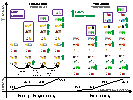
\includegraphics[width=0.7\textwidth]{figs/autolibra-teaser.pdf}
    \caption{Caption}
    \label{fig:enter-label}
\end{wrapfigure}

The Extraction Step of AutoLibra is designed to extract metrics from human feedback and agent trajectories.


With AutoLibra, we aim to answer the following research questions:
\begin{itemize}
    \item \textbf{RQ1:} Can LLMs serve as a proxy for humans when being used in agent behavior thematic analysis,
    behavior evaluation, and meta-evaluating the LLM-as-a-Judge results?
    \item \textbf{RQ2:} What are the differences between the metrics induced by AutoLibra and the behavior evaluation
    metrics designed by human experts?
    \item \textbf{RQ3:} Is AutoLibra useful for improving the performance of agents in different tasks by 
    providing fine-grained behavior evaluation for human agent engineers and agent learning algorithms?
\end{itemize}





\section{AutoLibra\protect
\includegraphics[height=1em]{figs/scale.png}}


\section{The lens \protect
\includegraphics[height=1em]{figs/microscope.png}: Agent evaluation with AutoLibra}
\section{The ladder \protect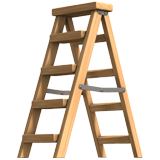
\includegraphics[height=1em]{figs/ladder.png}: Agent improvement with AutoLibra}

Methods
Improvements
Prompt
Failed attempts
Scores
Defeat null hypothesis of:
- Goal score alone being sufficient
- Human-derived metrics alone being sufficient

(~2 pages total incl. tables, shortened prompts)

Turn 0:
\begin{wraptable}[19]{r}{0.60\textwidth} % 'r' for right, adjust the width as needed
\centering
\small
\vspace{-30pt}
\begin{tabular}{ccl}
\toprule
\multicolumn{1}{c}{Emoji}& 
\multicolumn{1}{c}{It.} & 
\multicolumn{1}{l}{Metric} \\
\midrule
\rowcolor{gray!10} 
\includegraphics[scale=0.07]{figs/emojis/emoji_1.png} & 0 & Win Condition Recognition \\
\midrule
\rowcolor{gray!10} 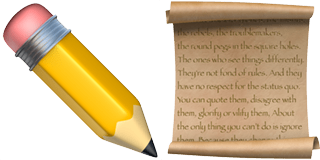
\includegraphics[scale=0.07]{figs/emojis/emoji_2.png} & 0 & Rule Modification \\
\midrule
\rowcolor{gray!10} 
\includegraphics[scale=0.07]{figs/emojis/emoji_3.png} & 0 & Direct Navigation Efficiency \\
\midrule
\rowcolor{gray!10} 
\includegraphics[scale=0.07]{figs/emojis/emoji_4.png} & 0 & Context-Sensitive Decision Making \\
\midrule
\rowcolor{gray!30} 
\includegraphics[scale=0.07]{figs/emojis/emoji_5.png} & 1 & Win Rule Construction \\
\midrule
\rowcolor{gray!30} 
\includegraphics[scale=0.07]{figs/emojis/emoji_6.png} & 1 & Selective Interaction With Relevant Objects  \\
\midrule
\rowcolor{gray!30} 
\includegraphics[scale=0.07]{figs/emojis/emoji_7.png} & 1 & Rule Manipulation and Execution  \\
\midrule
\rowcolor{gray!60} 
\includegraphics[scale=0.07]{figs/emojis/emoji_8.png} & 2 & Subtask Coordination \\
\midrule
\rowcolor{gray!90} 
\includegraphics[scale=0.07]{figs/emojis/emoji_9.png} & 3 & Immovable Interaction \\
\bottomrule
\end{tabular}
\caption{Metrics and Turn of Induction \newline for Baba-Is-AI}
\label{tab:metrics}
\end{wraptable}

Metrics obtained are:
\begin{itemize}
    \item Win Condition Recognition (WCR)
    \item Rule Modification for Obstacle Management (RMO)
    \item Direct Navigation Efficiency (DNE)
    \item Context-Sensitive Decision Making (CSDM)
\end{itemize}
Win condition recognition prequisite to all other metrics, turn 1 improvements target this metric specifically.

Turn 0 trajectory appears stochastic, impossible for human to isolate model behaviors for targeted improvement; very low goal score/random trajectory makes using goal score as an agent improvement metric not useful in this case.

Turn 1 improvement and motivation:
\begin{enumerate}
    \item Few-shot prompting, targets WCR by giving model example of identifying win condition from native env observations
    \item Subtask-level planning guidance, target improvement of CSDM and WCR by mapping environment observations to goals, which model could not do in turn 0
\end{enumerate}

Turn 1:

\begin{itemize}
    \item Improvement in WCR vs Turn 0, indicating T1 improvements worked
    \item Slight improvement in RMO, DNE, CSDM but not statistically significant
    \item Overall improvement in BALROG score because agent seeks objectives
    \item Qualitatively, agent now targets specific blocks instead of randomly walking - but also now gets stuck when objective complex or multi-step
\end{itemize}

Metrics obtained are:
\begin{itemize}
    \item Win Rule Construction (WR)
    \item Selective Interaction with Relevant Objects (SI)
    \item Rule Manipulation and Execution (RME)
\end{itemize}

Turn 2 unsuccessful improvements (Decreased performance)
\begin{enumerate}
    \item 1-step location and action history as part of observation
    \item 5-step location and action history as part of observation
    \item Movement templates (given a start location and destination, what movements are necessary to navigate without colliding with obstacles)
\end{enumerate}

Turn 2 improvement and motivation:
\begin{enumerate}
    \item Augment subtask-level planning instructions with positional instructions, targets RME and RMO
    \item Meta-prompting by providing condition-based task identification heuristic, targets SI, WCR, and WR
    \item Augment few-shot example with movement guidance
\end{enumerate}


Turn 2:


\begin{itemize}
    \item Substantial improvement in WCR due to more detailed, condition-based task identification heuristic, corresponding increase in other metrics supports idea that WCR is prerequisite metric to other reasoning metrics
    \item Strong increase in RME and RMO, indicating improved agent reasoning performance induced by more detailed subtask-level planning  
    \item SI no improvement, agent still misunderstands map directions and confuses rule blocks with objects
    \item Qualitatively, agent now recognizes when wall needs to be broken and breaks wall rule; still cannot assemble rules to win; still gets stuck on immovable blocks and walls
\end{itemize}

Metrics obtained are:
\begin{itemize}
    \item Subtask Coordination and Overall Task Planning (SC)
\end{itemize}

Turn 3 improvement and motivation:
\begin{enumerate}
    \item Format observations as absolute position (as opposed to relative), listing of immovable/movable blocks (DNE)
    \item Chain-of-thought reasoning to assemble goal agenda based on turn-to-turn observations (SC)
    \item Many-shot example of task solving and goal agenda formation (SC, RME)
    \item Navigation instructions to avoid undesired block and wall collisions (DNE)
    \item Explicit instructions on how to assemble rules (WR, RME)
\end{enumerate}

Turn 3:

\begin{itemize}
    \item Large increase in SI and CSDM induced by agent following instructions in CoT reasoning plan.
    \item Strong improvement in DNE, DNE metric informed addition of absolute position and navigation instructions
    \item Small increase in WR; agent demonstrates limited capabilities to assemble win condition rules as long as few other obstacles present
    \item Qualitatively, nearly agent always understands when wall rule can be and cannot be broken, as well as when it's not necessary to break the wall rule, covers nearly all tasks that involve going to win; understands how to assemble win rules but still struggles with changing block direction and understanding that blocks get stuck against walls

\end{itemize}

Metrics obtained are:
\begin{itemize}
    \item Interaction with Immovable Objects (IO)
\end{itemize}

\subsection{Style}

Papers to be submitted to COLM 2025 must be prepared according to the
instructions presented here.

%% Please note that we have introduced automatic line number generation
%% into the style file for \LaTeXe. This is to help reviewers
%% refer to specific lines of the paper when they make their comments. Please do
%% NOT refer to these line numbers in your paper as they will be removed from the
%% style file for the final version of accepted papers.

Authors are required to use the COLM \LaTeX{} style files obtainable at the
COLM website. Please make sure you use the current files and
not previous versions. Tweaking the style files may be grounds for rejection.

\subsubsection{Copy Options}

If your paper is ultimately accepted, the option {\tt
  {\textbackslash}final} should be set  for the {\tt {\textbackslash}usepackage[submission]\{colm2025\_conference\}} command for the camera ready version. The {\tt submission} options is the default, and is to be used for all submissions during the review process. It also turns on the line numbers. If you wish to submit a preprint, the option {\tt preprint} should be used.
  
  

\subsection{Retrieval of style files}

The style files for COLM and other conference information are available online at:
\begin{center}
   \url{http://www.colmweb.org/}
\end{center}
The file \verb+colm2025_conference.pdf+ contains these
instructions and illustrates the
various formatting requirements your COLM paper must satisfy.
Submissions must be made using \LaTeX{} and the style files
\verb+colm2025_conference.sty+ and \verb+colm2025_conference.bst+ (to be used with \LaTeX{}2e). The file
\verb+colm2025_conference.tex+ may be used as a ``shell'' for writing your paper. All you
have to do is replace the author, title, abstract, and text of the paper with
your own.

The formatting instructions contained in these style files are summarized in
sections \ref{gen_inst}, \ref{headings}, and \ref{others} below.

\section{General formatting instructions}
\label{gen_inst}

The text must be confined within a rectangle 5.5~inches (33~picas) wide and
9~inches (54~picas) long. The left margin is 1.5~inch (9~picas).
Use 10~point type with a vertical spacing of 11~points. Palatino is the
preferred typeface throughout, and is mandatory for the main text. Paragraphs are separated by 1/2~line space, with no indentation. 

Paper title is 17~point and left-aligned.
All pages should start at 1~inch (6~picas) from the top of the page.

Please verify that any custom header information you may add does not override the style defined in this document. This has been known to occur especially when submissions are converted to a new template from a previous one (i.e., for re-submission to a different venue). 

Authors' names are
set in boldface, and each name is placed above its corresponding
address. The lead author's name is to be listed first, and
the co-authors' names are set to follow. Authors sharing the
same address can be on the same line.

Please pay special attention to the instructions in section \ref{others}
regarding figures, tables, acknowledgements, and references.


There will be a strict upper limit of 9 pages for the main text of the initial submission, with unlimited additional pages for citations. 

We strongly recommend following arXiv's guidelines for making your paper friendly for HTML conversion: \url{https://info.arxiv.org/help/submit_latex_best_practices.html}.


\section{Headings: first level}
\label{headings}

First level headings are in lower case (except for first word and proper nouns), bold face,
flush left and in point size 12. One line space before the first level
heading and 1/2~line space after the first level heading.

\subsection{Headings: second level}

Second level headings are in lower case (except for first word and proper nouns), bold face,
flush left and in point size 10. One line space before the second level
heading and 1/2~line space after the second level heading.

\subsubsection{Headings: third level}

Third level headings are in lower case (except for first word and proper nouns), bold face, italics, 
flush left and in point size 10. One line space before the third level
heading and 1/2~line space after the third level heading.

\section{Citations, figures, tables, references}\label{others}

These instructions apply to everyone, regardless of the formatter being used.

\subsection{Citations within the text}

Citations within the text should be based on the \texttt{natbib} package
and include the authors' last names and year (with the ``et~al.'' construct
for more than two authors). When the authors or the publication are
included in the sentence, the citation should not be in parenthesis using \verb|\citet{}| (as
in ``See \citet{Vaswani+2017} for more information.''). Otherwise, the citation
should be in parenthesis using \verb|\citep{}| (as in ``Transformers are a key tool
for developing language models~\citep{Vaswani+2017}.'').

The corresponding references are to be listed in alphabetical order of
authors, in the \textsc{References} section. As to the format of the
references themselves, any style is acceptable as long as it is used
consistently.

\subsection{Footnotes}

Indicate footnotes with a number\footnote{Sample of the first footnote} in the
text. Place the footnotes at the bottom of the page on which they appear.
Precede the footnote with a horizontal rule of 2~inches
(12~picas).\footnote{Sample of the second footnote}

\subsection{Figures}

All artwork must be neat, clean, and legible. Lines should be dark
enough for purposes of reproduction; art work should not be
hand-drawn. Any text within the figure must be readable. We ask to not use font sizes below {\tt small}. We strongly recommend to use vector representations (e.g., pdf or svg) for all diagrams. 
We strongly recommend positioning all figures at the top or bottom of the page.

The figure number and caption always appear below the figure. Place one line space before the figure caption, and one line space after the figure. The figure caption is lower case (except for first word and proper nouns); figures are numbered consecutively.
Make sure the figure caption does not get separated from the figure.
Leave sufficient space to avoid splitting the figure and figure caption.

You may use color figures.
However, it is best for the
figure captions and the paper body to make sense if the paper is printed
either in black/white or in color.
\begin{figure}[t]
\begin{center}
%\framebox[4.0in]{$\;$}
\fbox{\rule[-.5cm]{0cm}{4cm} \rule[-.5cm]{4cm}{0cm}}
\end{center}
\caption{Sample figure caption.}
\end{figure}

\subsection{Tables}

All tables must be centered, neat, clean and legible. Do not use hand-drawn tables. The table number and title always appear below the table. See Table~\ref{sample-table}. Please do not use font sizes below {\tt small} in tables. We recommend using {\tt booktabs} or a similar package to style tables. 
We strongly recommend positioning all tables at the top or bottom of the page.

Place one line space before the table title, one line space after the table title, and one line space after the table. The table title must be lowercase (except for first word and proper nouns); tables are numbered consecutively.

\begin{table}[t]
\begin{center}
\begin{tabular}{ll}
\toprule
\multicolumn{1}{c}{\bf PART}  &\multicolumn{1}{c}{\bf DESCRIPTION} \\
\midrule
Dendrite         &Input terminal \\
Axon             &Output terminal \\
Soma             &Cell body (contains cell nucleus) \\
\bottomrule
\end{tabular}
\end{center}
\caption{Sample table title}\label{sample-table}
\end{table}




\section{Final instructions}
Do not change any aspects of the formatting parameters in the style files.
In particular, do not modify the width or length of the rectangle the text
should fit into, and do not change font sizes (except perhaps in the
\textsc{References} section; see below). Please note that pages should be
numbered.

\section{Preparing PostScript or PDF files}

Please prepare PostScript or PDF files with paper size ``US Letter'', and
not, for example, ``A4''. The -t
letter option on dvips will produce US Letter files.

Consider directly generating PDF files using \verb+pdflatex+
(especially if you are a MiKTeX user).
PDF figures must be substituted for EPS figures, however.

Otherwise, please generate your PostScript and PDF files with the following commands:
\begin{verbatim}
dvips mypaper.dvi -t letter -Ppdf -G0 -o mypaper.ps
ps2pdf mypaper.ps mypaper.pdf
\end{verbatim}

\subsection{Margins in LaTeX}

Most of the margin problems come from figures positioned by hand using
\verb+\special+ or other commands. We suggest using the command
\verb+\includegraphics+
from the graphicx package. Always specify the figure width as a multiple of
the line width as in the example below using .eps graphics
\begin{verbatim}
   \usepackage[dvips]{graphicx} ...
   \includegraphics[width=0.8\linewidth]{myfile.eps}
\end{verbatim}
or % Apr 2009 addition
\begin{verbatim}
   \usepackage[pdftex]{graphicx} ...
   \includegraphics[width=0.8\linewidth]{myfile.pdf}
\end{verbatim}
for .pdf graphics.
See section~4.4 in the graphics bundle documentation (\url{http://www.ctan.org/tex-archive/macros/latex/required/graphics/grfguide.ps})

A number of width problems arise when LaTeX cannot properly hyphenate a
line. Please give LaTeX hyphenation hints using the \verb+\-+ command.

\section*{Author Contributions}
If you'd like to, you may include  a section for author contributions as is done
in many journals. This is optional and at the discretion of the authors.

\section*{Acknowledgments}
Use unnumbered first level headings for the acknowledgments. All
acknowledgments, including those to funding agencies, go at the end of the paper.

\section*{Ethics Statement}
Authors can add an optional ethics statement to the paper. 
For papers that touch on ethical issues, this section will be evaluated as part of the review process. The ethics statement should come at the end of the paper. It does not count toward the page limit, but should not be more than 1 page. 



\bibliography{colm2025_conference}
\bibliographystyle{colm2025_conference}

\appendix
\section{Appendix}
You may include other additional sections here.

\end{document}
